% kapitel5.tex
\definecolor{light-gray}{gray}{0.93}
\chapter{Evaluation an simulierten Datensätzen} \label{sec:eval}

\section{Simulation und Workflow-Run} \label{sec:sim}

Zur Evaluation wurde durch das Tool ddRAGE \cite{timm_2018, ddrage} ein simulierter Testdatensatz \cite{testdata} von ddRADSeq-Daten für drei Individuen erzeugt. Der Testdatensatz umfasst 6965 single-end Reads mit 100 Basenpaaren Readlänge für 50 Loci und mit Mutationswahrscheinlichkeiten von 0.8999 für Substitutionen, 0.05 für Insertionen und 0.05 für Deletionen. DdRAGE liefert neben verschiedenen zusätzlichen Informationen zur Simulation auch die Sequenzen der simulierten Loci. Zur Evaluation sollen diese mit den durch NodeRAD identifizierten Loci verglichen werden.\\

Für die Analyse mit NodeRAD wurde eine Heterozygotiewahrscheinlichkeit von jeweils 0.01 für Substitutionen, Insertionen und Deletionen festgelegt. Die Sequenzierfehlerrate für Substitutionen $L_{sub}$ wurde für über die geschätzte Fehlerrate $p_{i}$ der Basenqualität der Reads bestimmt (siehe Kap. \ref{pHMM_alleles}). Für Indels wurden empirisch ermittelte Sequenzierfehlerraten der Illumina Sequenzierplattformen \cite{schirmer_2016} verwendet. Diese in der Konfigurationsdatei festgelegten Konstanten sowie die angewendeten Schwellenwerte des Workflow-Runs sind in Tab. \ref{tbl:config} aufgelistet. \\

\begin{table}[H]
	\begin{center}
		\begin{tabular}{lccc}
			\hline
			\multicolumn{4}{|c|}{\cellcolor{light-gray}\textbf{Konfigurierte Schwellenwerte}} \\ \hline \hline
			\multicolumn{1}{|c|}{\textbf{\begin{tabular}[c]{@{}c@{}}threshold max \\ edit distance\end{tabular}}} & \multicolumn{2}{c|}{\textbf{treshold-seq-noise}} & \multicolumn{1}{c|}{\textbf{treshold-cluster-size}} \\ \hline \hline
			\multicolumn{1}{|l|}{} & \multicolumn{1}{c|}{small-clusters} & \multicolumn{1}{c|}{large-clusters} & \multicolumn{1}{l|}{} \\ \hline
			\multicolumn{1}{|c|}{9} & \multicolumn{1}{c|}{2} & \multicolumn{1}{c|}{4} & \multicolumn{1}{c|}{300} \\ \hline
			\multicolumn{4}{l}{} \\ \hline
			\multicolumn{4}{|c|}{\cellcolor{light-gray}\textbf{Konfigurierte Konstanten}} \\ \hline \hline
			\multicolumn{1}{|l|}{} & \multicolumn{1}{c|}{\textbf{insertion}} & \multicolumn{1}{c|}{\textbf{deletion}} & \multicolumn{1}{c|}{\textbf{substitution}} \\ \hline
			\multicolumn{1}{|l|}{\textbf{error-per-base}} & \multicolumn{1}{c|}{$ 2.8 \, \cdotp 10^{-6} $} & \multicolumn{1}{c|}{$ 5.1 \, \cdotp 10^{-6} $} & \multicolumn{1}{c|}{$L_{i} = \frac{1}{3} \; \cdotp \; p_{i}$} \\ \hline
			\multicolumn{1}{|l|}{\textbf{heterozygosity}} & \multicolumn{1}{c|}{0.01} & \multicolumn{1}{c|}{0.01} & \multicolumn{1}{c|}{0.01} \\ \hline
		\end{tabular}
	\caption{Konfiguration des Workflow-Runs.}
	\label{tbl:config}
	\end{center}
\end{table}	

Für jedes der drei Individuen $A$, $B$ und $C$ wurden durch NodeRAD die wahrscheinlichsten Loci ermittelt und mit den Sequenzen der tatsächlich simulierten Loci aus den Zusatzinformationen von ddRAGE verglichen. Der Vergleich erfolgte durch das Tool BLAST (Basic Local Alignment Search Tool) \cite{altschul_1990}. Hierfür wurden sowohl die Loci der Simualtion als auch die Resultate des Workflows in das FASTA-Format geparsed. Hierbei wurden für die simulierten Loci auch die jeweiligen Mutationen der Individuen auf die Loci-Sequenzen gemapped. \\


Um die Daten lokal gegeneinander zu vergleichen wurde anschließend für die Loci der Simulation eine BLAST-Datenbank erzeugt. Gegen diese Datenbank erfolgte dann die BLAST-Analyse mit den identifizierten Loci des Workflows. Aus den Ergebnissen der BLAST-Analyse wurden anschließend verschiedene Plots in der Programmiersprache R erzeugt, die Kap. \ref{sec:res} zu finden sind. Die Regeln und Scripte der Evaluation sind in NodeRAD integriert und können über die Konfigurationsdatei durch Angabe eines Pfades zu den durch ddRAGE simulierten Loci im yaml-Format aktiviert werden.

\section{Ergebnisse} \label{sec:res}

Die simulierten RADSeq-Daten zeigten in der FastQ-Analyse eine gute Qualität der Basen (\autoref{fig:basequal}) und wiesen nach dem Trimming keine Adaptersequenzen mehr auf (\autoref{fig:adapt}).\\

\begin{figure}[H]
	\begin{center}
		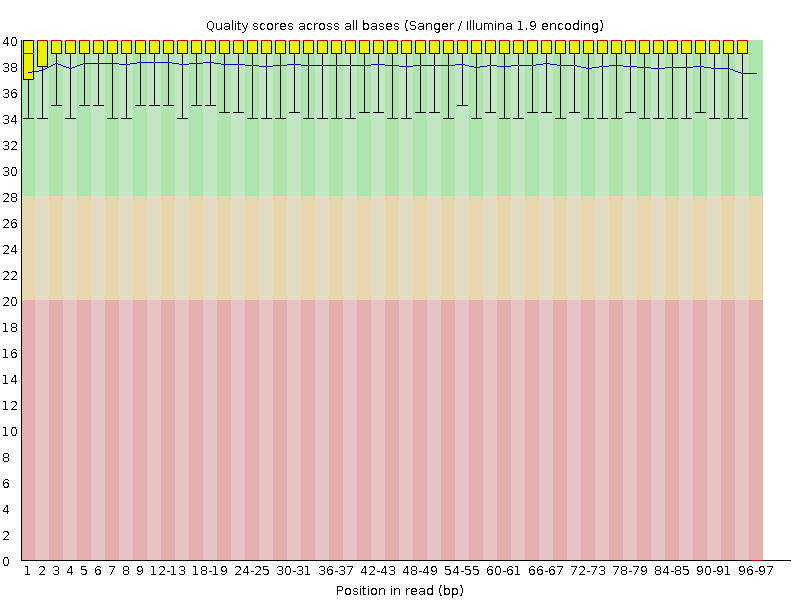
\includegraphics[height=10cm]{bilder/evaluation/fastq/per_base_quality.png}
		\caption{FastQ-Analyse: Basenqualität der Readsequenzen von Individuum A.}
		\label{fig:basequal}
	\end{center}
\end{figure}
\vspace{-2cm}
\begin{figure}[H]
	\begin{center}
		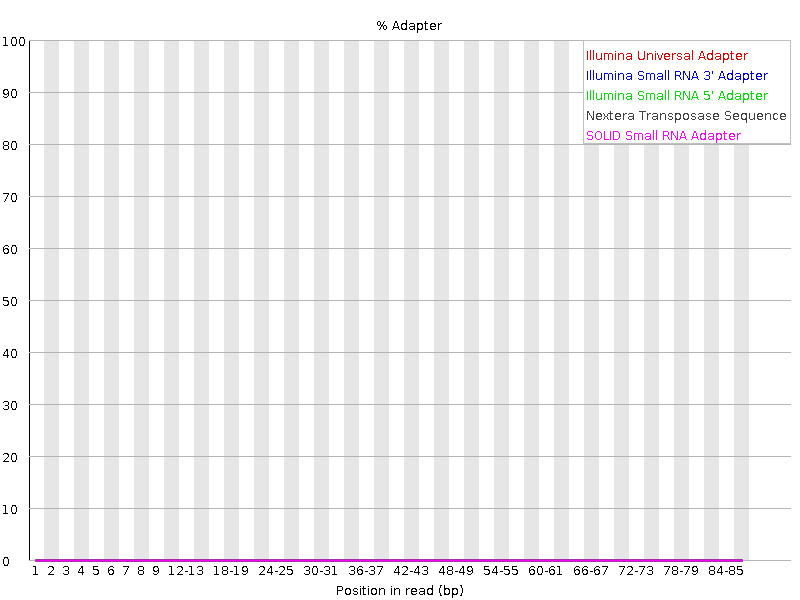
\includegraphics[height=10cm]{bilder/evaluation/fastq/adapter_content.png}
		\caption{FastQ-Analyse: Adaptergehalt der Reads von Individuum A nach dem Trimming durch Cutadapt.}
		\label{fig:adapt}
	\end{center}
\end{figure}

Bei den jeweils 50 Loci der ddRAGE-Simulation, kommen bei Individuum A eine homozygote und vier heterzygote Mutataionen durch Substitution vor. Individuum B weist an drei Loci homozygote und an einem Locus eine heterozygote Substition auf. Individuum C besitzt drei homozygote Mutationen. Die BLAST-Analyse soll Aufschluss über die Genauigkeit geben, mit der NodeRAD in der Lage ist die Loci und die Varianten mit Mutationen zu finden. Für eine bessere Übersichtlichkeit werden in diesem Kapitel nur die Plots zur BLAST-Analyse von Individuum A exemplarisch dargestellt, da hier ein höherer Anteil heterozygoter Mutationen vorliegt. Sämtliche Plots für die Individuen B und C können jedoch im Anhang eingesehen werden (siehe Kap. \ref{append_plots}) und zeigen keine relevanten Abweichungen gegenüber den Plots von Individuum A.\\

Beim BLAST-Algorithmus werden die Nukleotidsequenzen der durch NodeRAD identifizierten Loci gegen die tatsächlich simulierten Loci paarweise verglichen \cite{gaedeke_2007}. Das resultierende Sequenzalignment gibt die besten Übereinstimmungen (Hits) an. Die Ähnlichkeit jedes Sequenzpaares wird über den prozentualen Anteil identischer Nukleotide ausgedrückt (Identität). Wie in \autoref{fig:a-ident} und \autoref{fig:a-hist} erkennbar, sind die meisten Loci aus der Analyse mit NodeRAD identisch zu den tatsächlich simulierten Loci. Bei denjenigen Loci, die eine geringere Sequenzähnlichkeit aufweisen, handelt es sich um zusätzliche Allele die NodeRAD zu dem betreffenden Locus identifiziert hat. Dort liegt ein Mismatch zur tatsächlichen und korrekt identifizierten Sequenz von maximal einer Base vor. Lediglich bei Individuum C wurde ein Locus mit einem Mismatch von einer Base falsch bestimmt ohne dass zusätzliche Allele mit der korrekten Locussequenz identifiziert wurden. Nur wenige Loci wurden durch NodeRAD gar nicht gefunden. Insgesamt wurden bei Individuum A 44 der 50 Loci gefunden, bei Individuum B konnten 48 und bei Individuum C 47 Loci identifiziert werden (siehe auch Tab ....).\\

\newpage

\begin{figure}[H]
	\begin{center}
		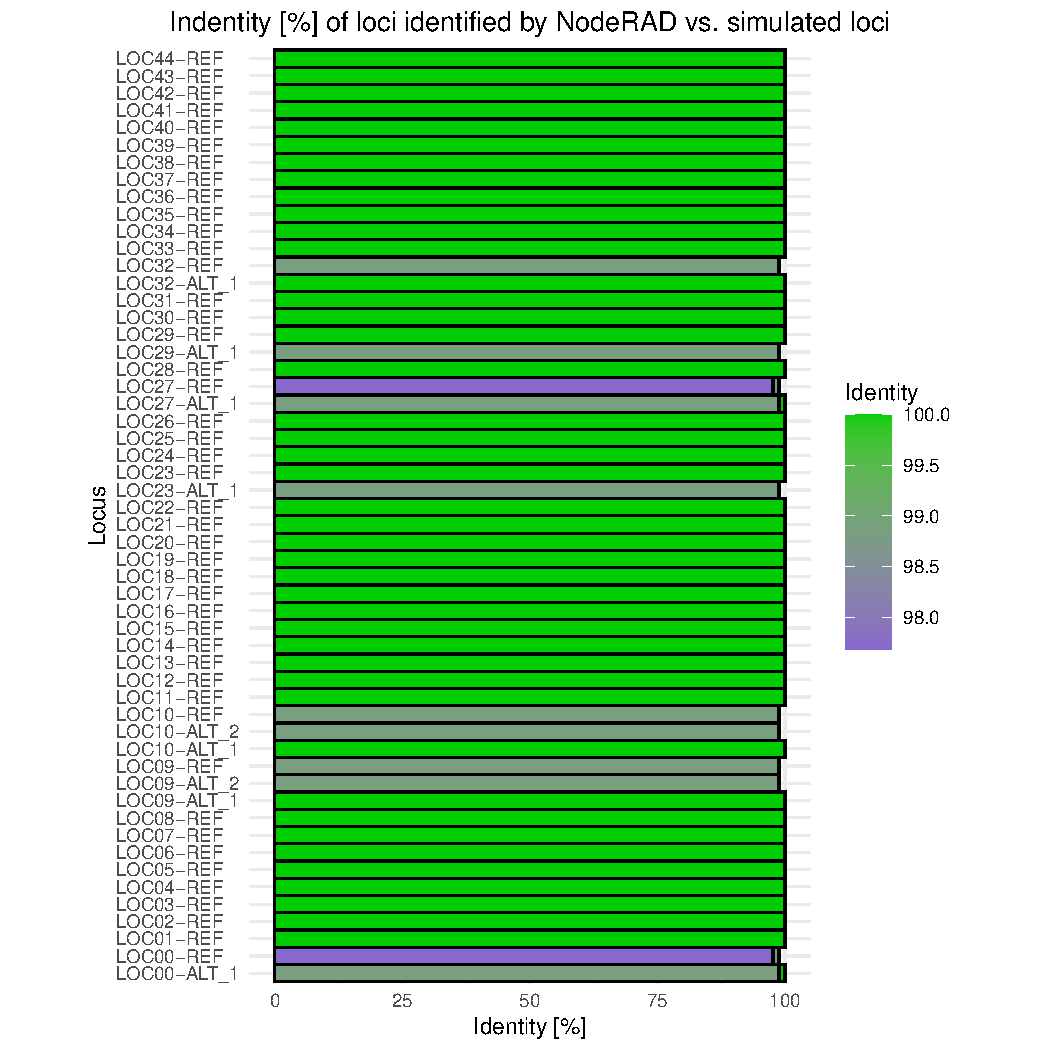
\includegraphics[height=16cm]{bilder/evaluation/perc_ident/A.plot_loci.pdf}
		\caption{Individuum A: Sequenzähnlichkeit (Identität in $ \% $) der durch NodeRAD bestimmten Allele gegenüber den simulierten Allelen.}
		\label{fig:a-ident}
	\end{center}
\end{figure}

\begin{figure}[H]
	\begin{center}
		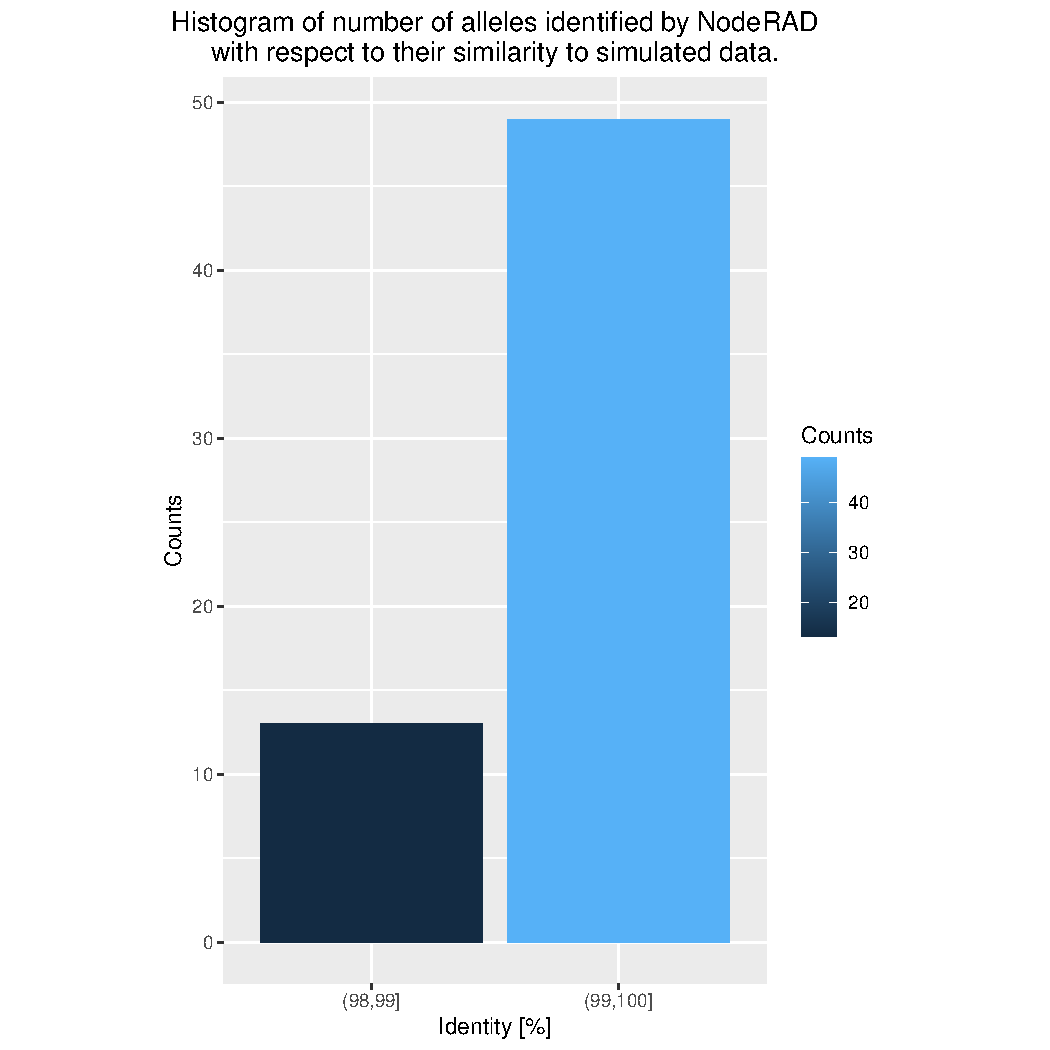
\includegraphics[height=12cm]{bilder/evaluation/hist_perc_ident/A.plot_hist.pdf}
		\caption{Individuum A: Anzahl der durch NodeRAD bestimmten Allele hinsichtlich der Sequenzählichkeit (Identität in $ \% $) zu den simulierten Allelen}
		\label{fig:a-hist}
	\end{center}
\end{figure}


Bei der BLAST-Analyse werden zudem beim Vergleich der Nukleotidsequenzen Werte für jedes Match bzw. Mismatch vergeben \cite{gaedeke_2007}. Die Summe dieser Werte stellt den Rohwert-Score des Sequenzaligments dar. Aus diesem Score lassen sich zwei statische Merkmale der BLAST-Analyse ableiten: der E-Value und der Bitscore. \\

Der E-Value (expectation value) ist ein Signifikanzmaß und beschreibt die Anzahl zufälliger Treffer mit mindestens dem betrachteten Score, die bei gegebener Größer der Referenzdatenbank zu erwarten wären \cite{gaedeke_2007}. Je kleiner der E-Value ist, desto geringer ist die Wahrscheinlichkeit, dass ein Hit nur zufällig gefunden wurde. Bei allen Individuen weisen die Hits eine hohe Signifikanz auf (siehe \autoref{fig:a-eval}). Lediglich bei einem Hit findet sich eine wesentlich geringere Signifikanz. Diese Abweichung betrifft bei allen Individuen den selben Locus der ddRAGE-simulierten Daten. Das korrespondierende durch NodeRAD bestimmte Allel ist deutlich verkürzt, so dass dieser Ausreißer am ehesten auf ein fehlerhaftes Adaptertrimming zurückzuführen ist.\\

\begin{figure}[H]
	\begin{center}
		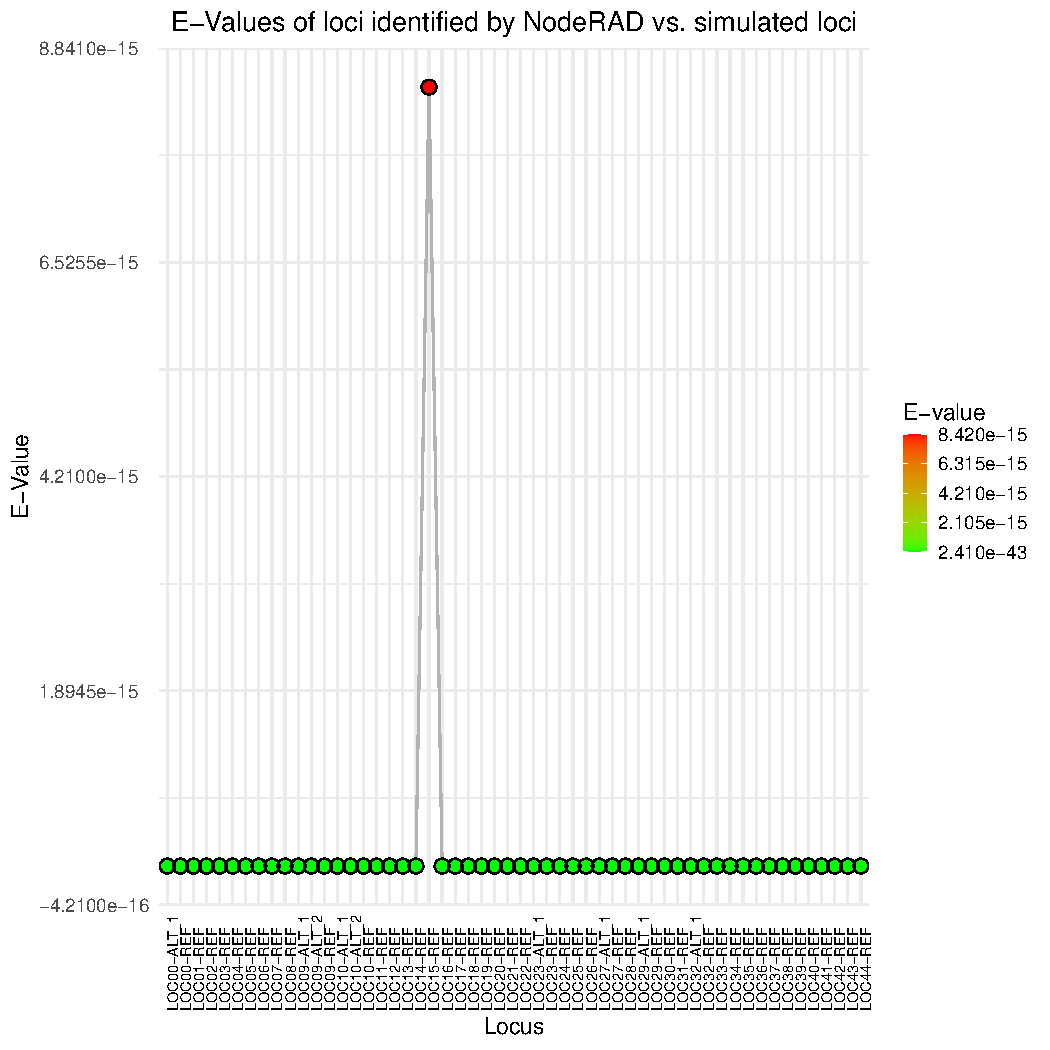
\includegraphics[height=16cm]{bilder/evaluation/evalues/A.plot_evalues.pdf}
		\caption{Individuum A: E-Values aus dem Vergleich der durch NodeRAD bestimmten Allele mit den simulierten Allelen}
		\label{fig:a-eval}
	\end{center}
\end{figure}

Der Bitscore ist der normalisierte Wert des Rohwert-Scores \cite{gaedeke_2007}. Durch die Normalisierung können die einzelnen Alignments mit einander hinsichtlich ihres Scores verglichen werden. Je höher Wert des Bitscores liegt, desto besser ist die Sequenzübereinstimmung. Auch hier weisen bis auf den bereits erwähnten Ausreißer mit verkürzter Sequenz sämtliche durch NodeRAD identifizierten Allele hohe Werte auf (siehe \autoref{fig:a-bitscore}).

\begin{figure}[H]
	\begin{center}
		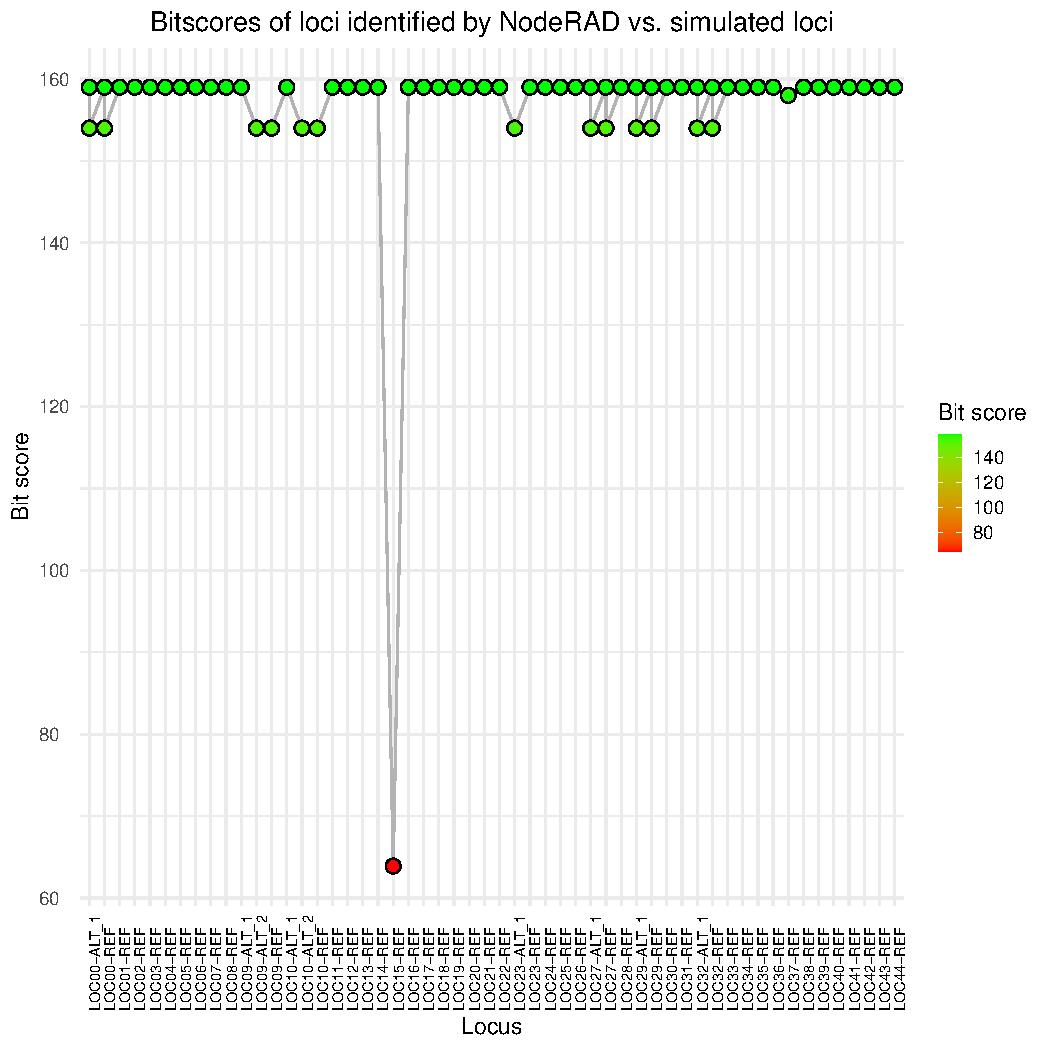
\includegraphics[height=16cm]{bilder/evaluation/bitscores/A.plot_bitscores.pdf}
		\caption{Individuum A: Bitscores aus dem Vergleich der durch NodeRAD bestimmten Allele mit den simulierten Allelen}
		\label{fig:a-bitscore}
	\end{center}
\end{figure}

Im Hinblick auf die Loci-Zuordnung durch NodeRAD wurden sämtliche homo- und heterozygoten Mutationen bei allen Individuen korrekt identifiziert. Bis auf einen falsch identifizierten Locus bei Individuum C und wenige fehlende Loci (siehe oben), wurden auch die meisten Allele der homozygoten Loci ohne Varianten gefunden. Hier fanden sich allerdings auch einige Loci, bei denen NodeRAD einen heterozygoten Locus unter Beteiligung eines weiteren Allels definierte, obwohl der tatsächliche Locus homozygot ist. Bei diesen falsch-heterozygoten Loci wiesen die zusätzlich dem Locus zugeordneten Allele ein Mismatch von jeweils einer Base auf. Insgesamt waren bei allen Individuen solche falsch-heterozygoten Loci detektiert worden. Falsch-homozygote Loci fanden sich dagegen nicht (siehe Tab. ).



\let\cleardoublepage\clearpage